\documentclass[12pt,a4paper]{article}

% ─── Page Layout ───────────────────────────────────────────────────────────────
\usepackage[a4paper, margin=0.8in, headheight=14pt]{geometry}

% ─── Fonts (XeLaTeX) ───────────────────────────────────────────────────────────
\usepackage{fontspec}
\usepackage{unicode-math}
\setmainfont{TeX Gyre Pagella}
\setmonofont[Scale=0.88]{TeX Gyre Cursor}
\setmathfont{Latin Modern Math}

% ─── Packages ──────────────────────────────────────────────────────────────────
\usepackage{xcolor}
\usepackage{colortbl}
\usepackage{titlesec}
\usepackage{enumitem}
\usepackage{tabularx}
\usepackage{booktabs}
\usepackage{array}
\usepackage{amsmath}
\usepackage{tikz}
\usetikzlibrary{shapes.geometric, arrows.meta, positioning, calc, fit, decorations.pathreplacing}
\usepackage{tcolorbox}
\tcbuselibrary{skins, breakable}
\usepackage{hyperref}
\usepackage{fancyhdr}
\usepackage{graphicx}
\usepackage{microtype}
\hyphenpenalty=10000
\exhyphenpenalty=10000
\sloppy
\usepackage{caption}
\usepackage{setspace}
\usepackage{multirow}
\usepackage{tocloft}

% ─── Q&A helper ────────────────────────────────────────────────────────────────
\newcommand{\Q}[1]{\textbf{#1}\par\noindent\ignorespaces}

% ─── Colour Palette ────────────────────────────────────────────────────────────
\definecolor{myred}{RGB}{196,30,58}
\definecolor{mydark}{RGB}{30,30,50}
\definecolor{mygreen}{RGB}{14,120,80}
\definecolor{myteal}{RGB}{0,130,140}
\definecolor{myamber}{RGB}{180,100,0}
\definecolor{mypurple}{RGB}{100,30,160}
\definecolor{mygray}{RGB}{246,247,249}
\definecolor{mgframe}{RGB}{180,185,200}
\definecolor{watermark}{RGB}{145,150,170}
\definecolor{hdrred}{RGB}{250,232,235}
\definecolor{hdrgreen}{RGB}{220,244,233}
\definecolor{hdrteal}{RGB}{220,242,244}
\definecolor{hdramber}{RGB}{253,242,215}
\definecolor{hdrpurple}{RGB}{238,228,255}
\definecolor{hdrgray}{RGB}{238,240,245}
\definecolor{rowalt}{RGB}{250,251,253}

% ─── Section Formatting ────────────────────────────────────────────────────────
\titleformat{\section}
  {\large\bfseries\color{myred}}{\thesection.}{0.5em}{}
  [\vspace{1pt}{\color{myred}\rule{\linewidth}{0.8pt}}]
\titleformat{\subsection}
  {\normalsize\bfseries\color{myteal}}{\thesubsection}{0.5em}{}
\titlespacing*{\section}{0pt}{18pt}{7pt}
\titlespacing*{\subsection}{0pt}{11pt}{4pt}

% ─── Paragraph ─────────────────────────────────────────────────────────────────
\setlength{\parindent}{0pt}
\setlength{\parskip}{4pt}

% ─── TOC Styling ───────────────────────────────────────────────────────────────
\renewcommand{\cfttoctitlefont}{\large\bfseries\color{myred}}
\renewcommand{\cftaftertoctitle}{\par\noindent{\color{myred}\rule{\linewidth}{0.8pt}}}
\setlength{\cftbeforetoctitleskip}{0pt}
\setlength{\cftaftertoctitleskip}{6pt}
\renewcommand{\cftsecfont}{\normalsize\bfseries\color{mydark}}
\renewcommand{\cftsecpagefont}{\normalsize\bfseries\color{mydark}}
\renewcommand{\cftsecleader}{\cftdotfill{\cftdotsep}}
\setlength{\cftbeforesecskip}{7pt}
\renewcommand{\cftsubsecfont}{\small\color{mydark}}
\renewcommand{\cftsubsecpagefont}{\small\color{mydark}}
\setlength{\cftbeforesubsecskip}{3pt}
\setlength{\cftsubsecindent}{1.4em}

% ─── Table helpers ─────────────────────────────────────────────────────────────
\renewcommand{\arraystretch}{1.45}
\setlength{\tabcolsep}{6pt}
\arrayrulecolor{mydark}
\newcolumntype{B}[1]{>{\small\bfseries\raggedright\arraybackslash}m{#1}}
\newcolumntype{Y}{>{\small\raggedright\arraybackslash}X}
\renewcommand{\tabularxcolumn}[1]{m{#1}}

% ─── Header / Footer ───────────────────────────────────────────────────────────
\pagestyle{fancy}
\fancyhf{}
\fancyhead[L]{\small\color{myred}\textbf{PE-EC701A}\;\color{mydark}--- Microwave Theory and Technique}
\fancyhead[R]{\small\color{myteal}\textbf{Module 3 Notes}}
\fancyfoot[C]{\small\color{mydark}\thepage}
\fancyfoot[R]{\small\color{watermark}\textit{\copyright\ Biraj}}
\renewcommand{\headrulewidth}{0.5pt}
\renewcommand{\footrulewidth}{0.3pt}

% ─── Hyperref ──────────────────────────────────────────────────────────────────
\hypersetup{
  colorlinks=true, linkcolor=myteal, urlcolor=myteal,
  pdfauthor={Biraj Sarkar},
  pdftitle={PE-EC701A --- Module 3 Notes}
}

% ─── tcolorbox styles ──────────────────────────────────────────────────────────
\tcbset{
  tikzbox/.style={
    colback=mygray, colframe=mgframe, boxrule=0.6pt, arc=4pt,
    left=8pt, right=8pt, top=6pt, bottom=6pt,
    colbacktitle=mgframe, coltitle=mydark,
    fonttitle=\small\bfseries
  },
  defbox/.style={
    colback=hdrgreen, colframe=mygreen, boxrule=0.8pt, arc=4pt,
    left=9pt, right=9pt, top=6pt, bottom=6pt,
    colbacktitle=mygreen, coltitle=white,
    fonttitle=\small\bfseries
  },
  formulabox/.style={
    colback=hdrteal, colframe=myteal, boxrule=0.8pt, arc=4pt,
    left=9pt, right=9pt, top=7pt, bottom=7pt,
    colbacktitle=myteal, coltitle=white,
    fonttitle=\small\bfseries
  },
  examplebox/.style={
    colback=hdramber, colframe=myamber, boxrule=0.8pt, arc=4pt,
    left=9pt, right=9pt, top=6pt, bottom=6pt,
    colbacktitle=myamber, coltitle=white,
    fonttitle=\small\bfseries
  },
  masonbox/.style={
    colback=hdrpurple, colframe=mypurple, boxrule=0.8pt, arc=4pt,
    left=9pt, right=9pt, top=6pt, bottom=6pt,
    colbacktitle=mypurple, coltitle=white,
    fonttitle=\small\bfseries
  },
  exambox/.style={
    colback=hdrpurple, colframe=mypurple, boxrule=1pt, arc=5pt,
    left=10pt, right=10pt, top=8pt, bottom=8pt,
    colbacktitle=mypurple, coltitle=white,
    fonttitle=\bfseries,
    breakable, title after break={\textbf{Frequently Asked / Viva Questions (contd.)}}}
}
% Make all boxes breakable across pages
\tcbset{breakable}

% ─── TikZ styles ───────────────────────────────────────────────────────────────
\tikzset{
  block/.style={rectangle, draw=myteal, fill=hdrteal,
    text width=2.4cm, align=center, minimum height=0.95cm,
    font=\small, rounded corners=3pt, line width=0.7pt},
  redblock/.style={rectangle, draw=myred, fill=hdrred,
    text width=2.4cm, align=center, minimum height=0.95cm,
    font=\small, rounded corners=3pt, line width=0.7pt},
  netnode/.style={rectangle, draw=myteal, fill=hdrteal,
    text width=1.5cm, align=center, minimum height=0.8cm,
    font=\small, rounded corners=3pt, line width=0.7pt},
  sumjunc/.style={circle, draw=myamber, fill=hdramber,
    minimum size=0.62cm, font=\small, line width=0.8pt},
  snode/.style={circle, draw=mypurple, fill=hdrpurple,
    minimum size=0.55cm, font=\footnotesize, line width=0.7pt},
  arrow/.style={-Stealth, thick, color=mydark},
  redarrow/.style={-Stealth, thick, color=myred},
  line/.style={thick, color=mydark}
}

% ═══════════════════════════════════════════════════════════════════════════════
\begin{document}
% ═══════════════════════════════════════════════════════════════════════════════

\begin{center}
  {\LARGE\bfseries\color{myred} PE-EC701A --- Microwave Theory and Technique}\\[5pt]
  {\normalsize\color{mydark} Semester VII \quad$\bullet$\quad 3L:0T:0P \quad$\bullet$\quad 3 Credits}\\[3pt]
  {\normalsize\color{myteal}\textbf{Module 3 Exam Notes: RF and Microwave Transmission Lines}}\\[3pt]
  {\small\color{mydark} CGEC \;$|$\; B.Tech ECE (2023--27) \;$|$\; \textit{Biraj Sarkar}}
\end{center}
\vspace{2pt}
\noindent{\color{myred}\rule{\linewidth}{1.5pt}}
\vspace{2pt}

\hypersetup{linkcolor=mydark}
\tableofcontents
\hypersetup{linkcolor=myteal}
\newpage

% ===============================================================================
\section{Coaxial Line}
% ===============================================================================

The coaxial line is a standard TEM transmission line with two concentric circular conductors. It operates from DC up to frequencies where higher-order waveguide modes (usually $\text{TE}_{11}$) begin to propagate.

\begin{tcolorbox}[tikzbox, title={Coaxial Line Structure}]
\begin{minipage}[c]{0.45\linewidth}
\centering
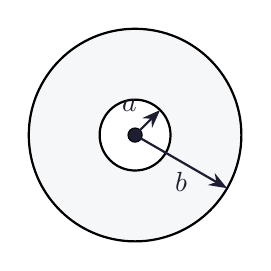
\begin{tikzpicture}[scale=0.9]
  \draw[thick, fill=mygray] (0,0) circle (1.5cm);
  \draw[thick, fill=white] (0,0) circle (0.5cm);
  \draw[fill=mydark] (0,0) circle (0.1cm);
  
  \draw[arrow] (0,0) -- (45:0.5) node[midway, above left] {$a$};
  \draw[arrow] (0,0) -- (-30:1.5) node[midway, below] {$b$};
\end{tikzpicture}
\end{minipage}\hfill
\begin{minipage}[c]{0.5\linewidth}
\raggedright
\textbf{Conductors:}\\[3pt]
Inner Radius = $a$\\
Outer Radius = $b$\\
Dielectric constant = $\epsilon_r$
\end{minipage}
\end{tcolorbox}

\begin{tcolorbox}[formulabox, title={\textbf{Coaxial Line Characteristic Impedance}}]
The characteristic impedance $Z_0$ of a lossless coaxial line is given by:
\begin{equation}
  Z_0 = \frac{\eta_0}{2\pi \sqrt{\epsilon_r}} \ln\left(\frac{b}{a}\right) \approx \frac{138}{\sqrt{\epsilon_r}} \log_{10}\left(\frac{b}{a}\right) \quad (\Omega)
\end{equation}
Where:
\begin{itemize}[leftmargin=1.5em, itemsep=1pt, topsep=2pt]
  \item[] $\eta_0 \approx 377\,\Omega$ is the intrinsic impedance of free space.
  \item[] $\epsilon_r$ is the relative permittivity of the dielectric.
\end{itemize}
\end{tcolorbox}

% ===============================================================================
\section{Rectangular Waveguide}
% ===============================================================================

A rectangular waveguide is a hollow metallic pipe of rectangular cross-section. Since it has only one conductor, it cannot support TEM waves; propagation occurs via TE and TM modes.

\begin{tcolorbox}[tikzbox, title={Rectangular Waveguide Geometry}]
\begin{minipage}[c]{0.52\linewidth}
\centering
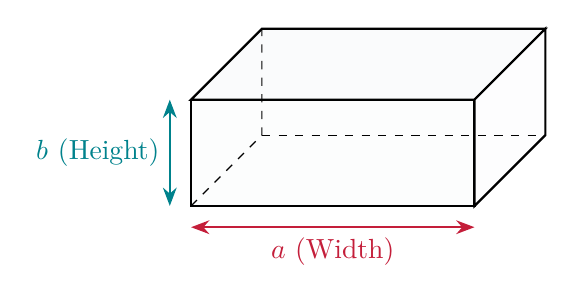
\begin{tikzpicture}[scale=0.9]
  % Draw 3D-like rectangular waveguide
  \draw[thick, fill=mygray!50] (0,0) -- (4,0) -- (5,1) -- (1,1) -- cycle;
  \draw[thick, fill=mygray!30] (0,-1.5) -- (4,-1.5) -- (4,0) -- (0,0) -- cycle;
  \draw[thick, fill=mygray!20] (4,-1.5) -- (5,-0.5) -- (5,1) -- (4,0) -- cycle;
  
  % Inner dotted lines for back boundaries
  \draw[dashed] (0,-1.5) -- (1,-0.5) -- (1,1);
  \draw[dashed] (1,-0.5) -- (5,-0.5);
  
  % Dimension indicators
  \draw[Stealth-Stealth, thick, color=myred] (0,-1.8) -- (4,-1.8) node[midway, below] {$a$ (Width)};
  \draw[Stealth-Stealth, thick, color=myteal] (-0.3,-1.5) -- (-0.3,0) node[midway, left] {$b$ (Height)};
\end{tikzpicture}
\end{minipage}\hfill
\begin{minipage}[c]{0.43\linewidth}
\raggedright
\textbf{Dominant dimension relation:}\\[3pt]
$a > b$\\[2pt]
Typically, $a = 2b$ to maximize single-mode bandwidth.
\end{minipage}
\end{tcolorbox}

\subsection{Wave Equations and Mode Cutoff}
From Helmholtz wave equations inside a lossless rectangular guide:
\begin{equation}
  f_c = \frac{v_0}{2} \sqrt{\left(\frac{m}{a}\right)^{\!2} + \left(\frac{n}{b}\right)^{\!2}} = \frac{c}{2\sqrt{\epsilon_r}} \sqrt{\left(\frac{m}{a}\right)^{\!2} + \left(\frac{n}{b}\right)^{\!2}}
\end{equation}
Where $m$ and $n$ are mode integers. The \textbf{dominant mode} (lowest cutoff frequency) for $a > b$ is the \textbf{$\text{TE}_{10}$ mode} ($m=1, n=0$):
\begin{equation}
  f_{c(\text{TE}_{10})} = \frac{c}{2a\sqrt{\epsilon_r}}
\end{equation}

\subsection{Phase Velocity, Group Velocity, and Guide Wavelength}
Waveguide propagation constants vary non-linearly with frequency:
\begin{itemize}[leftmargin=*, itemsep=3pt]
  \item \textbf{Guide Wavelength ($\lambda_g$):} The distance between two equal-phase planes along the guide axis.
    \begin{equation}
      \lambda_g = \frac{\lambda_0}{\sqrt{1 - \left(\frac{f_c}{f}\right)^{\!2}}} > \lambda_0
    \end{equation}
  \item \textbf{Phase Velocity ($v_p$):} The velocity at which the wave's phase fronts propagate.
    \begin{equation}
      v_p = \frac{\omega}{\beta} = \frac{v_0}{\sqrt{1 - \left(\frac{f_c}{f}\right)^{\!2}}} > v_0
    \end{equation}
  \item \textbf{Group Velocity ($v_g$):} The velocity at which real energy or information travels.
    \begin{equation}
      v_g = \frac{d\omega}{d\beta} = v_0 \sqrt{1 - \left(\frac{f_c}{f}\right)^{\!2}} < v_0
    \end{equation}
\end{itemize}

\subsubsection{Derivation of the Velocity Relation}
We multiply the expressions for phase and group velocity:
\begin{equation*}
  v_p \cdot v_g = \left( \frac{v_0}{\sqrt{1 - (f_c/f)^2}} \right) \times \left( v_0 \sqrt{1 - (f_c/f)^2} \right) = v_0^2
\end{equation*}
In free space (air-filled waveguide), $v_0 = c$. Hence, we prove the fundamental relation:
\begin{equation}
  v_p \cdot v_g = c^2 \quad \text{(Q.E.D.)}
\end{equation}

% ===============================================================================
\section{Circular Waveguide}
% ===============================================================================

A circular waveguide is a hollow tube of circular cross-section. Solving the wave equations in cylindrical coordinates ($r, \phi, z$) requires Bessel functions.

\begin{tcolorbox}[tikzbox, title={Circular Waveguide Cross-Section}]
\begin{minipage}[c]{0.45\linewidth}
\centering
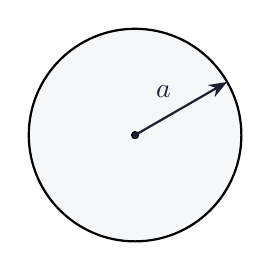
\begin{tikzpicture}[scale=0.9]
  \draw[thick, fill=mygray] (0,0) circle (1.5cm);
  \draw[fill=mydark] (0,0) circle (0.05cm);
  \draw[arrow] (0,0) -- (30:1.5) node[midway, above left] {$a$};
\end{tikzpicture}
\end{minipage}\hfill
\begin{minipage}[c]{0.5\linewidth}
\raggedright
\textbf{Cutoff Frequency Formula:}\\[3pt]
$f_c = \frac{p'_{mn} c}{2\pi a}$ \quad (for TE modes)\\[2pt]
$f_c = \frac{p_{mn} c}{2\pi a}$ \quad (for TM modes)\\[4pt]
Dominant Mode is \textbf{$\text{TE}_{11}$}, where $p'_{11} \approx 1.8412$.
\end{minipage}
\end{tcolorbox}

% ===============================================================================
\section{Stripline and Microstrip Line}
% ===============================================================================

Striplines and microstrip lines are planar transmission lines fabricated on dielectric substrates, forming the core of Microwave Integrated Circuits (MICs).

\begin{tcolorbox}[tikzbox, title={Planar Line Geometries (Stripline vs. Microstrip)}]
\centering
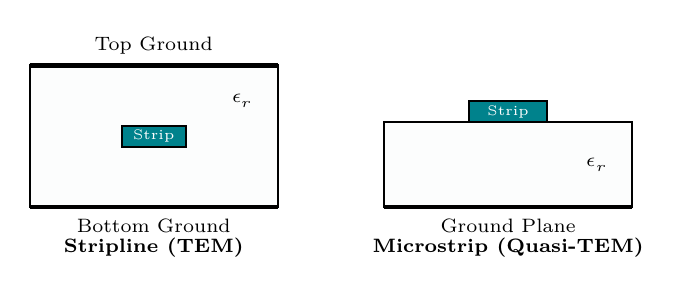
\begin{tikzpicture}[scale=0.9]
  % Stripline
  \draw[thick, fill=mygray!30] (-4,-1) rectangle (-0.5,1);
  \draw[line width=1.5pt] (-4,1) -- (-0.5,1) node[midway, above, font=\scriptsize] {Top Ground};
  \draw[line width=1.5pt] (-4,-1) -- (-0.5,-1) node[midway, below, font=\scriptsize] {Bottom Ground};
  \draw[thick, fill=myteal] (-2.7,-0.15) rectangle (-1.8,0.15) node[midway, font=\tiny\color{white}] {Strip};
  \node[below, font=\scriptsize\bfseries] at (-2.25,-1.3) {Stripline (TEM)};
  
  % Microstrip
  \draw[thick, fill=mygray!30] (1.0,-1.0) rectangle (4.5,0.2);
  \draw[line width=1.5pt] (1.0,-1.0) -- (4.5,-1.0) node[midway, below, font=\scriptsize] {Ground Plane};
  \draw[thick, fill=myteal] (2.2,0.2) rectangle (3.3,0.5) node[midway, font=\tiny\color{white}] {Strip};
  \node[below, font=\scriptsize\bfseries] at (2.75,-1.3) {Microstrip (Quasi-TEM)};
  
  % Labels
  \node[font=\scriptsize] at (-1,0.5) {$\epsilon_r$};
  \node[font=\scriptsize] at (4.0,-0.4) {$\epsilon_r$};
\end{tikzpicture}
\end{tcolorbox}

\subsection{Microstrip Design Formulas}
Because some electric field lines pass through air and others through the substrate, the wave propagation is \textbf{Quasi-TEM}. We define an \textbf{effective dielectric constant} ($\epsilon_{\text{eff}}$):
\begin{equation}
  \epsilon_{\text{eff}} = \frac{\epsilon_r + 1}{2} + \frac{\epsilon_r - 1}{2}\left(1 + 12\frac{h}{w}\right)^{\!-1/2}
\end{equation}
Where $w$ is the strip width and $h$ is substrate thickness. The characteristic impedance is:
\begin{equation}
  Z_0 = \frac{60}{\sqrt{\epsilon_{\text{eff}}}} \ln\left( 8\frac{h}{w} + \frac{w}{4h} \right) \quad \left(\text{for } w/h \le 1\right)
\end{equation}

% ===============================================================================
% MANDATORY QUICK REVISION PAGE
% ===============================================================================
\newpage
\begin{center}
  {\large\bfseries\color{myred} Quick Revision --- Module III}\\[3pt]
  {\small\color{mydark} RF and Microwave Transmission Lines $|$ PE-EC701A}
\end{center}
\noindent{\color{myred}\rule{\linewidth}{1.2pt}}
\vspace{4pt}

\begin{tcolorbox}[formulabox, title={\textbf{Key Formulas at a Glance}}]
\renewcommand{\arraystretch}{1.3}
\begin{tabularx}{\linewidth}{B{4.5cm} X}
Coaxial impedance       & $Z_0 = \frac{138}{\sqrt{\epsilon_r}} \log_{10}(b/a)$ \\[4pt]
Rectangular cutoff      & $f_c = \frac{c}{2\sqrt{\epsilon_r}} \sqrt{(m/a)^2 + (n/b)^2}$ \\[4pt]
Guide wavelength        & $\lambda_g = \frac{\lambda_0}{\sqrt{1 - (f_c/f)^2}}$ \\[4pt]
Velocity relation       & $v_p \cdot v_g = c^2$ \quad (in air-filled guide) \\[4pt]
Circular cutoff         & $f_c = \frac{p'_{mn} c}{2\pi a}$ \quad ($\text{TE}_{11}$ dominant, $p'_{11}=1.8412$) \\[4pt]
Effective dielectric    & $\epsilon_{\text{eff}} \approx \frac{\epsilon_r + 1}{2} + \frac{\epsilon_r - 1}{2}(1 + 12h/w)^{-1/2}$
\end{tabularx}
\tcbset{colbacktitle=mygreen, coltitle=white}
\end{tcolorbox}

\begin{tcolorbox}[defbox, title={\textbf{One-Line Definitions}}]
\begin{itemize}[leftmargin=*, itemsep=2.5pt, topsep=0pt]
  \item \textbf{Guide Wavelength:} The axial wavelength of a wave propagating inside a waveguide.
  \item \textbf{Dominant Mode:} The propagation mode with the absolute lowest cutoff frequency.
  \item \textbf{Phase Velocity:} The rate at which the wave's constant-phase wavefronts propagate.
  \item \textbf{Group Velocity:} The speed at which energy and information travel down the line.
  \item \textbf{Quasi-TEM Mode:} A mode resembling TEM but containing small longitudinal fields due to dielectric boundaries.
  \item \textbf{Stripline:} A planar transmission line sandwiched symmetrically between two ground planes.
  \item \textbf{Microstrip:} A planar line on a dielectric substrate with a single bottom ground plane.
\end{itemize}
\end{tcolorbox}

\begin{tcolorbox}[exambox, title={\textbf{Frequently Asked / Viva Questions}}]
\begin{enumerate}[topsep=0pt, label=\textbf{Q\arabic*.}, itemsep=5pt]
  \item \Q{What is the dominant mode in rectangular waveguides and why?}
    The $\text{TE}_{10}$ mode. It has the lowest cutoff frequency ($f_c = c/2a$), meaning it can propagate over the widest single-mode bandwidth.
  \item \Q{Why does a rectangular waveguide act as a high-pass filter?}
    Because it only supports wave propagation above its cutoff frequency ($f > f_c$). Waves below cutoff are attenuated exponentially.
  \item \Q{Explain the relation between phase velocity, group velocity, and the speed of light.}
    In an air-filled guide, $v_p \cdot v_g = c^2$. Since $v_g < c$, the phase velocity $v_p$ must be greater than the speed of light ($v_p > c$).
  \item \Q{What is the dominant mode of a circular waveguide?}
    The $\text{TE}_{11}$ mode, with a cutoff parameter $p'_{11} \approx 1.8412$.
  \item \Q{Why are microstrip lines called Quasi-TEM lines?}
    Because the fields exist in two different mediums (air above, substrate below). The phase velocity mismatch prevents a pure TEM mode.
  \item \Q{How does the characteristic impedance of a coaxial cable depend on conductor sizes?}
    It is proportional to the logarithm of the ratio of the outer radius to inner radius ($Z_0 \propto \ln(b/a)$).
  \item \Q{Why are rectangular waveguides typically designed with $a = 2b$?}
    To maximize the frequency range over which only the dominant $\text{TE}_{10}$ mode propagates before the next mode ($\text{TE}_{20}$ or $\text{TE}_{01}$) turns on.
  \item \Q{What is the physical meaning of the effective dielectric constant ($\epsilon_{\text{eff}}$)?}
    It is the equivalent permittivity of a uniform medium that would produce the same phase velocity as the air-substrate microstrip system.
  \item \Q{What are the advantages of Striplines over Microstrip lines?}
    Striplines are shielded on both sides, which reduces radiation losses and provides better isolation against electromagnetic interference.
  \item \Q{What is the cutoff wavelength ($\lambda_c$) of the dominant mode in a rectangular waveguide?}
    $\lambda_c = 2a$ for the $\text{TE}_{10}$ mode.
  \item \Q{What is a mode chart?}
    A plot of cutoff frequencies for various modes versus waveguide dimensions, used to select optimal waveguide sizes.
  \item \Q{Under what condition does dispersion occur in transmission lines?}
    Dispersion occurs when the phase velocity of the propagating wave depends on frequency ($dv_p/df \ne 0$), causing signals of different frequencies to spread in time.
\end{enumerate}
\tcbset{colbacktitle=mgframe, coltitle=mydark}
\end{tcolorbox}

\begin{tcolorbox}[tikzbox, title={Comparison of Microwave Transmission Lines}]
\renewcommand{\arraystretch}{1.4}
\par\noindent
\begin{tabularx}{\linewidth}{|B{3.0cm}|Y|Y|Y|}
\hline
\rowcolor{hdrgray}
\textbf{Parameter} & \textbf{Coaxial Line} & \textbf{Rectangular Waveguide} & \textbf{Microstrip Line} \\
\hline
\textbf{Mode Supported} & TEM & TE, TM & Quasi-TEM (TE/TM at high f) \\
\hline
\rowcolor{rowalt}
\textbf{Cutoff Freq $f_c$} & $0$ (propagates DC) & $f_c = c/2a > 0$ & $0$ (propagates DC) \\
\hline
\textbf{Bandwidth} & Very wide & Moderate (between modes) & Very wide \\
\hline
\rowcolor{rowalt}
\textbf{Losses} & Moderate & Very low (no dielectric) & High (conductor + radiation) \\
\hline
\textbf{Power Capacity} & Moderate & High & Low \\
\hline
\end{tabularx}
\end{tcolorbox}

\end{document}
